\chapter{Receiver side}

In order to receive both nodes simultaneously, an Ezcap DVB-T FM DAB receiver is used, which contains the RTL2832 chip. The SDR dongle is connected to the computer by USB2.0, and the I\&Q data is imported using the GNU-Radio software. 

\section{Graphical view of the signal}
First, figure \ref{fig:gnuradio_waterfall} is obtained to measure the frequency offset. 
The left signal is produced by pijnacer, and should be at center frequency 432.990 mHz, but as we can see, it is actually received at 432.964 mHz. The difference is caused by the initial offsets of the transmitters, and the frequency offset of the VCO in the SDR. 

\begin{figure}[h]
\centering
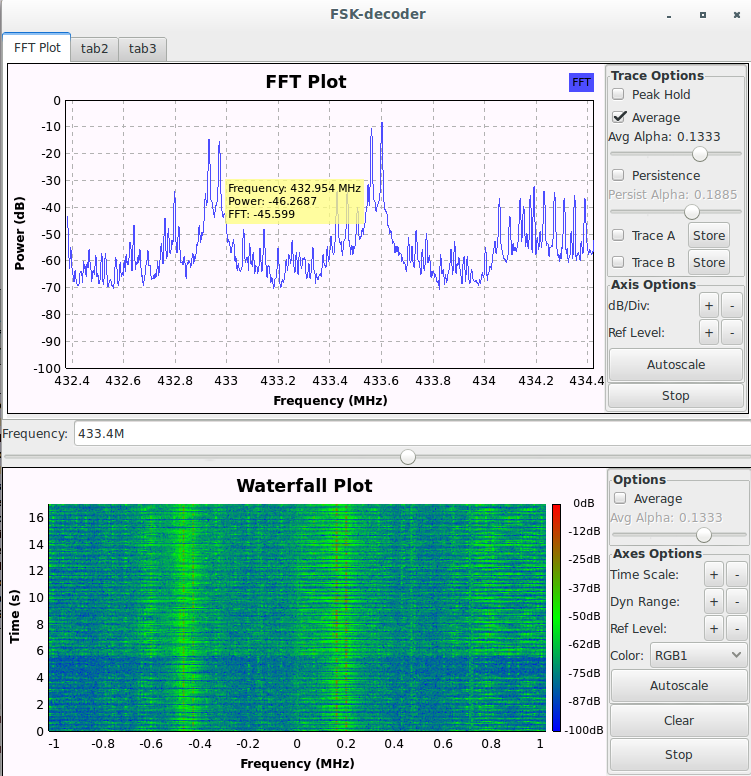
\includegraphics[width=0.7\linewidth]{figures/gnuradio_waterfall_catpure}
\caption{a gnu-radio capture of the frequency spectrum}
\label{fig:gnuradio_waterfall}
\end{figure}

In order to build the decoder efficiently, the FSK\_capture\_to\_file.grc is build, which contains a simple data sink block. The sampling frequency is set to 2.048 MSPS, which results in $2.048MSPS / 1200 baud \approx 1706 samples/symbol$. This is useful to know in order to perform a correct clock recovery later on.

The input data is measured with a center frequency 433.4. We'll take a graphical look at the recorded signal of both transmitters using the GNU radio flowchart depicted in \ref{fig:flowchart_play_from_file_grc}
\begin{figure}[h]
\centering
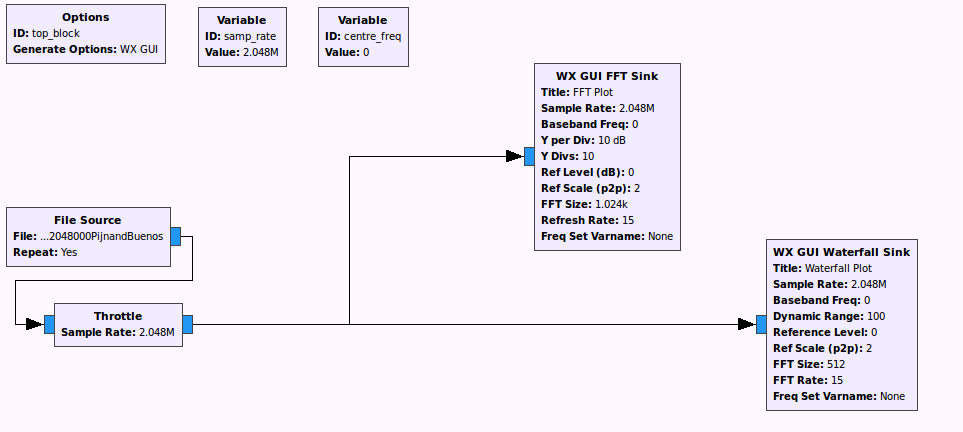
\includegraphics[width=0.7\linewidth]{figures/flowchart_play_from_file_grc}
\caption[gnu radio flowchart used to replay the captured data]{}

\label{fig:flowchart_play_from_file_grc}
\end{figure}

We expect that Pijnacker transmitting frequency is now 433.4 - 432.950 = 450 kHz below the current center frequency. Which is roughly shown in \ref{fig:gnuradio_waterfall_catpure_replay}. 

\begin{figure}[h]
\centering
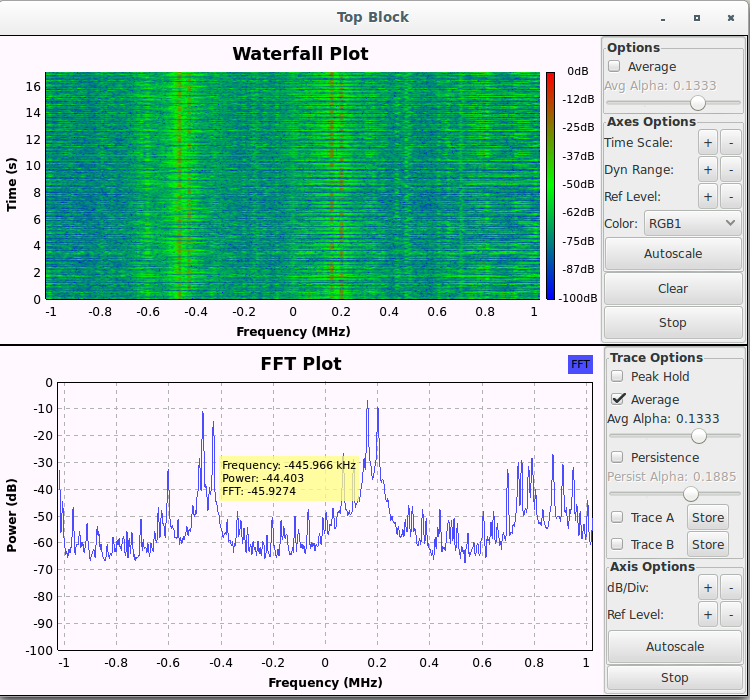
\includegraphics[width=0.7\linewidth]{figures/gnuradio_waterfall_catpure_replay}
\caption{replay of signal}
\label{fig:gnuradio_waterfall_catpure_replay}
\end{figure}
 
Once we replay the saved data using the file source block, the frequency of Pijnacker is at -450kHz, which can be seen in figure \ref{fig:gnuradio_waterfall_catpure_replay}. 

In order to decode the signal, the frequency is increased using a multiplier and an addition signal source block, with a frequency of 470 kHz. This sets the '0' at + 30kHz, and the '1' at 50 kHz. Then, the signal is passed through a low pass filter. The flowchart and the results are depicted in \ref{fig:pijnacker_isolated}.



\begin{figure}[ht]
\centering
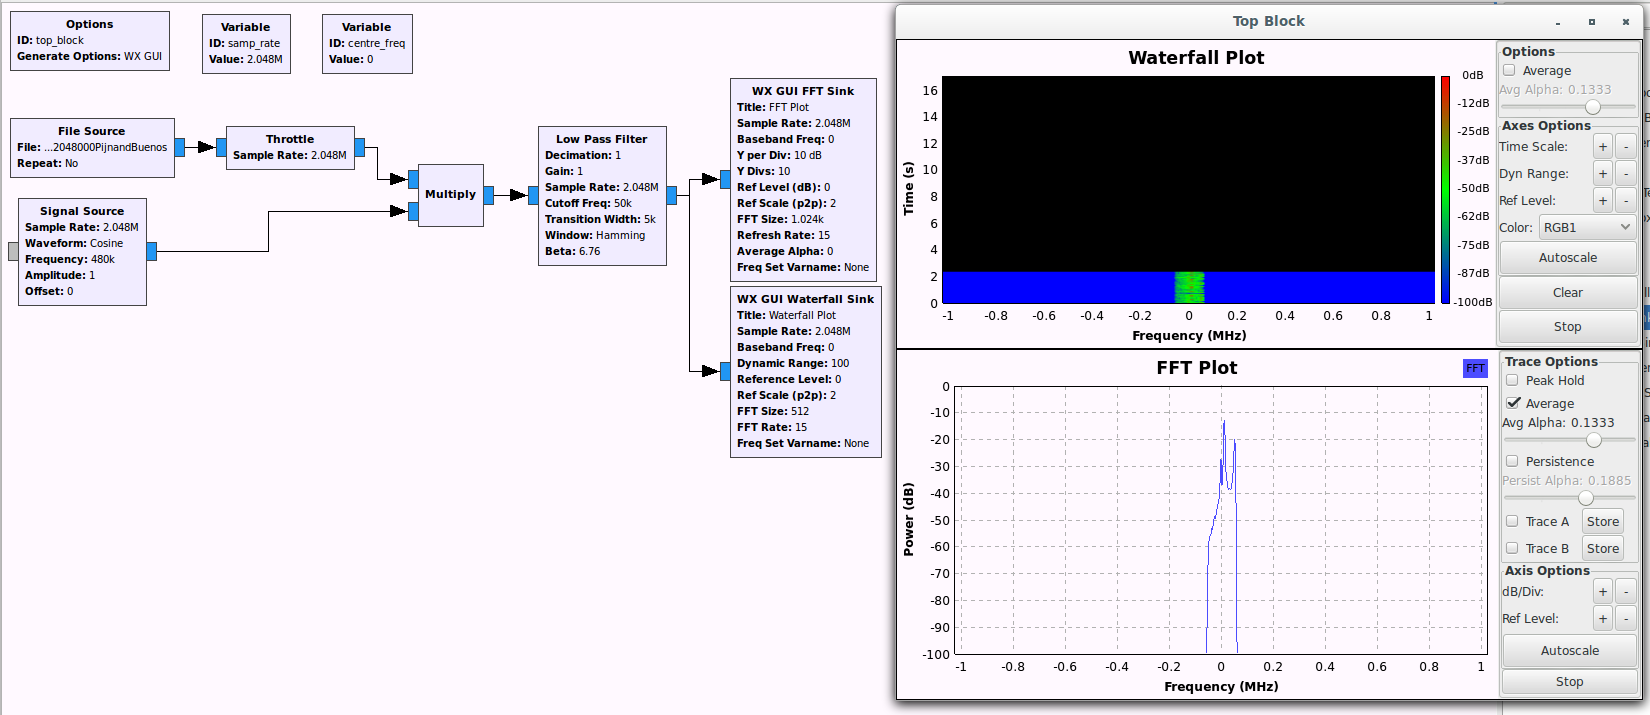
\includegraphics[width=1\linewidth]{figures/pijnacker_isolated}
\label{fig:pijnacker_isolated}
\end{figure}

From this point, we could use the GFSK decode block already availabe in the GNU-radio toolbox. However, this block only supports binairy data output which is unfortunately not easy readable. To gain a better understanding in the underlying principles, it is decided to use a quadratude demodulator, and look decode the signal in a binary AM fashion. After adding the quadrature demodulator, another low pas filter is used. with a cutt-off frequency of 1200 hertz. As the baudrate is 1200 symbols a second, and each symbol represents a binary '1' or a binary '0', we know that a signal representing a bit in AM can never be at a frequency higher than 1200 hertz. However, the filter is not infinitively steep, and therefor the cutoff frequency is set to 1100 hertz with a 800 hertz transition width. 

The flowchart and the output up to this point are depicted in figure \ref{fig:quaddemod_lowpas}. 


\begin{figure}[h]
\centering
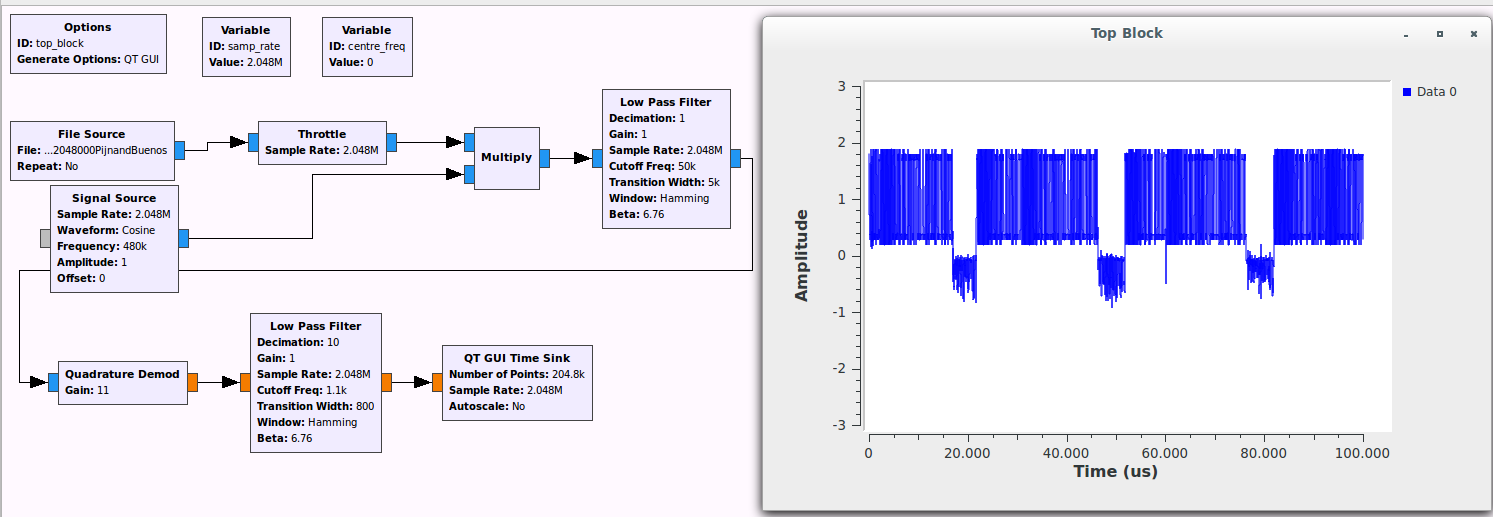
\includegraphics[width=1\linewidth]{figures/pijnacker_quadrature_demod}
\caption[quadrature demodulation]{Qaudrature demodulation with noise}
\label{fig:quaddemod_lowpas}
\end{figure}
 
 
To get rid of the noise in between the data frames, a simple threshold detector is used. The output of the threshold detector is multiplied with the output of the second low pass filer. Again, the flowchart and the result are depicted in \ref{fig:pijnacker_q_dem_improved}
 
 \begin{figure}[h]
\centering
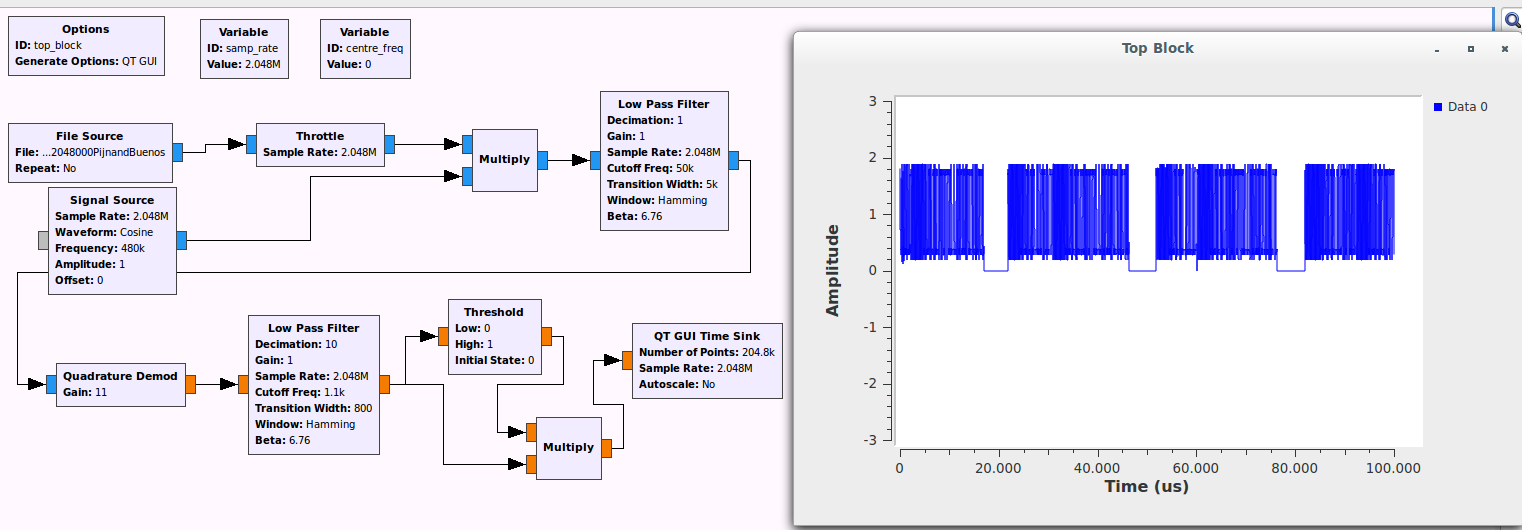
\includegraphics[width=1\linewidth]{figures/pijnacker_q_dem_improved}
\caption[pijnacker_q_dem_improved]{inter packet noise removed}
\label{fig:pijnacker_q_dem_improved}
\end{figure}

In order to recover the clock signal from the preamble, a Muller and Mueller clock recovery block $(Clock_recovery_MM)$ block is available in the toolbox. This block is not well documented, but the mailing list of gnu-radio provided the information necessary: \cite{GNU_MAILING_CLOCK_REC}

Omega: this is the expected number of samples per symbol (SPS) which is 1706
Gain omega: Control loop value indicating how fast adjustment in the omega value can be made. 
Mu: Initial estimate of the phase of the sample.
Gain mu: Control loop value indicating how fast adjustment in the mu value can be made. 
Omega Relative Limit: Percentage of maximal allowed omega deviation.

The output, after the clock recover block is show in \ref{fig:after_clock_rec}. Each positive value corresponds to a '1' being detected, a negative value corresponds to a '0' being detected. 

\begin{figure}[h]
\centering
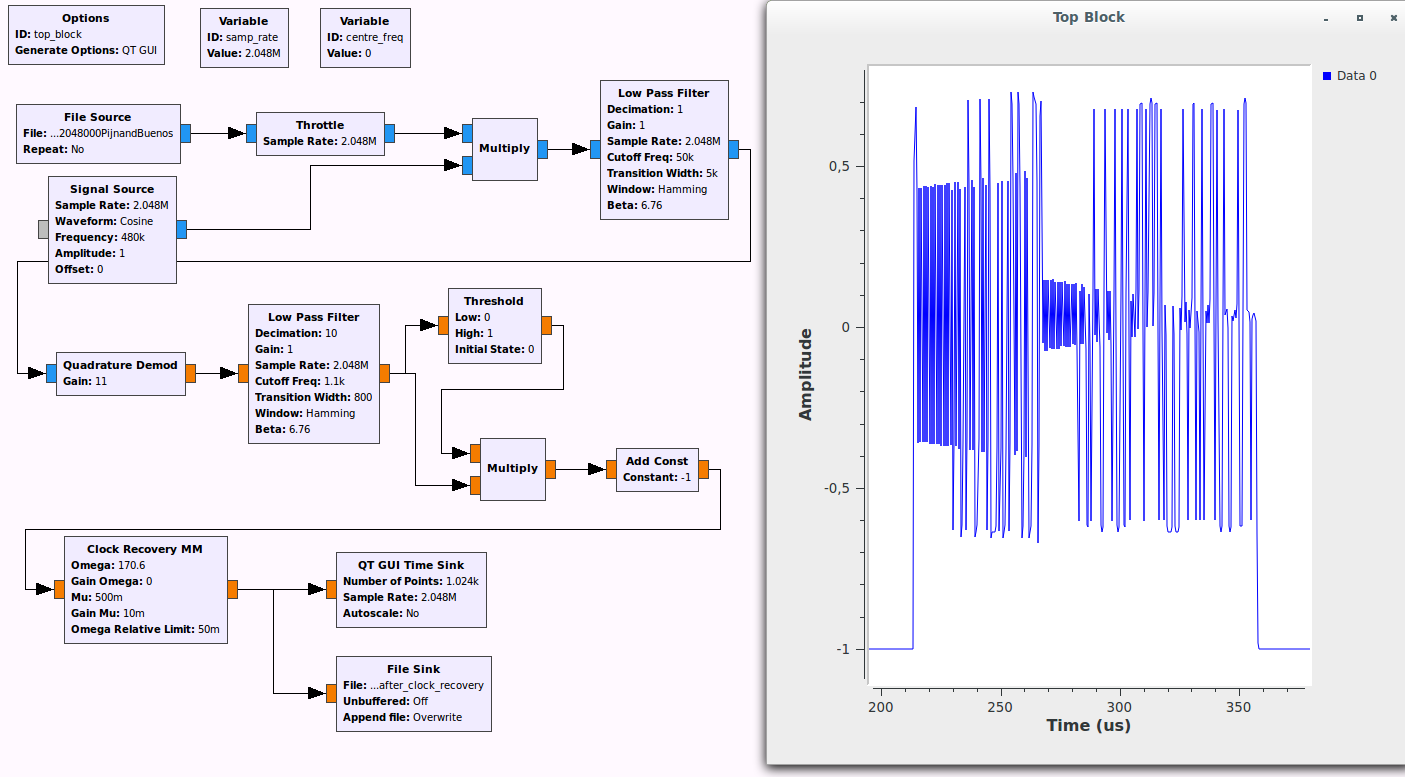
\includegraphics[width=1\linewidth]{figures/after_clock_rec}
\caption[Output after clock recovery]{data after clock recovery }
\label{fig:after_clock_rec}
\end{figure}


In order to clip the amplitude of this output to a '0' or a '1', the binary slicer is used. After the data is appropriately visible, we can add tags using the "correlate access code" tag block which we provide with the binairy representation of "TMCS". For convenience, the time raster sink block is added to display the data in a longer run. The output of this block is show in the bottom graph in \ref{fig:taggedburst}. Yellow represents a '1' bits detected, and in white the detection of a '0' bit is visible. Unfortunately, the default background color is also yellow. Note that the completely yellow block at the end actually indicates data that is not yet received. The graph on the top shows the tags as small red triangles. These are placed upon the bit stream by the correlate access block. 

\begin{figure}[h]
\centering
\includegraphics[width=1\linewidth]{"figures/tagged burst"}
\caption[tagged burst]{data after clock recovery, with amplitude correction and preamble tagging}
\label{fig:taggedburst}
\end{figure}


At this point, also the data is stored in the tagged file sink. The documentation of this block is unclear where the obtained files are actually located, but does specify that each block after a tag detection creates a new file. As this is not eligible for our goal, the author has decided to use the file obtained in fig \ref{fig:after_clock_rec} and write a own script in python to detect the preamble, and further decode the message offline. 

The python script "fsk\_decode\_to\_char" also implements a binary slicer, appends the '0' and '1' to a string, and searches this string for the data, which it extracts, converts to ascii characters, and outputs as data. 

The script skips the first two characters of the transmitted data. It is expected that this is due to the node identifier, as this is not jet taken into account.

[here i'll input the script, and the script output]

